%%%%%%%%%%%%%%%%%%%%%%%%%%%%%%%%%%%%%%%%%%%%%%%%%%%%%%%%%%%%%%%%%%%%%%%%%%%%%%%%%%%%%%%%%%
\begin{document}
\maketitle
%%%%%%%%%%%%%%%%%%%%%%%%%%%%%%%%%%%%%%%%%%%%%%%%%%%%%%%%%%%%%%%%%%%%%%%%%%%%%%%%%%%%%%%%%%

\begin{frame}
 \frametitle{Outline}
  \vspace{-1cm}
  1. Introduction\\[0.1cm]
  2. Mathematical Model\\[0.1cm]
  3. Validation\\[0.1cm]
  4. Results\\[0.1cm]
  5. Conclusion
\end{frame}


%%%%%%%%%%%%%%%%%%%%%%%%%%%%%%%%%%%%%%%%%%%%%%%%%%%%%%%%%%%%%%%%%%%%%%%%%%%%%%%%%%%%%%%%%

\begin{frame}
\frametitle{Introduction}
\vspace{-1.2cm}
\begin{columns}[c]
\column{.6\textwidth}
Motivation:
\begin{itemize}
  \item More people die from cardiovascular diseases that from any other cause in the world
\end{itemize}
 
\vspace{0.5cm}
 
Aims:
\begin{itemize}
 \justifying
 \item To know how the dynamics of blood flow in coronary artery with atherosclerosis
       and stent placed \\

 \vspace{0.2cm}
 \item To develop a Finite Element code for stream-vorticity formulation 
       with species transport equation

\end{itemize}
\column{.4\textwidth}
\begin{center}
  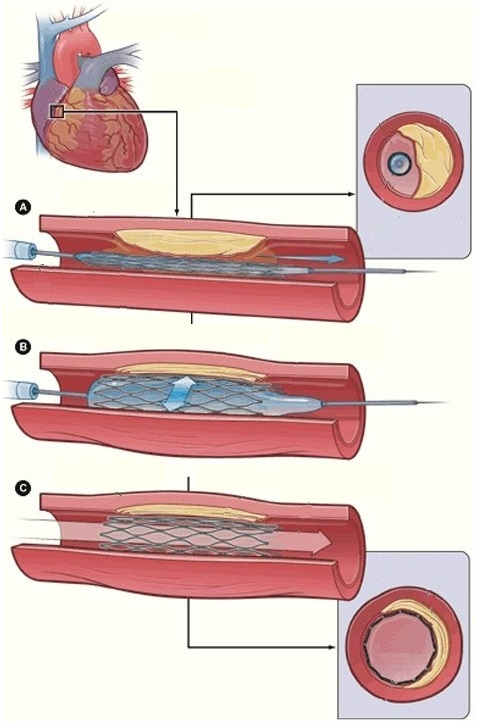
\includegraphics[scale=0.38]{images/stent_bare.jpg}
\end{center}
\end{columns}
\end{frame}


%%%%%%%%%%%%%%%%%%%%%%%%%%%%%%%%%%%%%%%%%%%%%%%%%%%%%%%%%%%%%%%%%%%%%%%%%%%%%%%%%%%%%%%%%%

\begin{frame}
  \vspace{-1cm}
  \textcolor{gray}{1. Introduction}\\[0.1cm]
  2. Mathematical Model\\[0.1cm]
  \textcolor{gray}{3. Validation}\\[0.1cm]
  \textcolor{gray}{4. Results}\\[0.1cm]
  \textcolor{gray}{5. Conclusion}
\end{frame}

%%%%%%%%%%%%%%%%%%%%%%%%%%%%%%%%%%%%%%%%%%%%%%%%%%%%%%%%%%%%%%%%%%%%%%%%%%%%%%%%%%%%%%%%%%

\begin{frame} 
 \frametitle{\Large Assumptions}
\vspace{-1cm}
\begin{center}
\begin{columns}[c]
\begin{column}{0.6\textwidth} 
\hspace{1cm}  1. Continuum hypothesis\\[0.1cm]
\hspace{1cm}  2. Homogeneous and Isotropic\\[0.1cm]
\hspace{1cm}  3. Incompressible\\[0.1cm]
\hspace{1cm}  4. Newtonian
\end{column}
\begin{column}{0.6\textwidth}
\hspace{0.5cm}  5. Constant Mass Difusivity\\[0.1cm]
\hspace{0.5cm}  6. Single-phase Flow\\[0.1cm]
\hspace{0.5cm}  7. Two-dimensional flow
\end{column}
\end{columns}
\end{center}
\small
\vspace{0.5cm}
\begin{equation*}
 \frac{\partial \omega}{\partial t} + \textbf{v} \cdot \nabla \omega = \frac{1}{Re} \nabla^{2} \omega
 \hspace{1.2cm}
 \nabla^{2} \psi = - \omega
\end{equation*}
\vspace{0.2cm}
\begin{equation*}
 \frac{\partial c}{\partial t} + \textbf{v} \cdot \nabla c = \frac{1}{ReSc} \nabla^{2} c
 \hspace{1.2cm}
 \textbf{v} = \textbf{D} \psi
\end{equation*}\\[0.8cm]

Where \textbf{D} is a differential operator
$\big[\partial / \partial y,- \partial / \partial x \big]$

\end{frame}


%%%%%%%%%%%%%%%%%%%%%%%%%%%%%%%%%%%%%%%%%%%%%%%%%%%%%%%%%%%%%%%%%%%%%%%%%%%%%%%%%%%%%%%%%%

\begin{frame} 
 \frametitle{\Large Finite Element Method}
\vspace{-1cm}
\begin{center}
\begin{columns}[c]
\begin{column}{1.2\textwidth} 
\begin{figure}[H]
\begin{center}
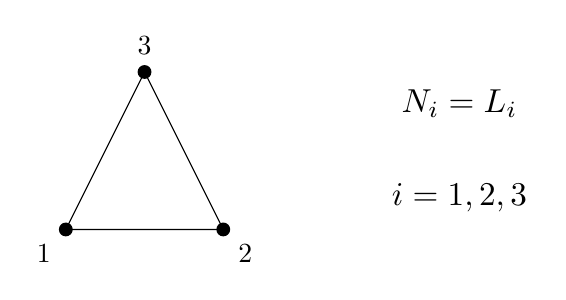
\begin{tikzpicture}[scale=2]
 \draw (0,0) -- (1,0) -- (0.5,1) -- cycle;

 \node[circle, fill=black, inner sep=0pt, minimum size=5pt,label=below left:{1}] at (0,0) {};
 \node[circle, fill=black, inner sep=0pt, minimum size=5pt,label=below right:{2}] at (1,0) {};
 \node[circle, fill=black, inner sep=0pt, minimum size=5pt,label=above:{3}] at (0.5,1) {};
 
 \node[draw=none, scale=1.2] at (2.5,0.8) {$N_i = L_i$};
 \node[draw=none, scale=1.2] at (2.5,0.2) {$i = 1,2,3$};
\end{tikzpicture}
\end{center}
\end{figure}
\end{column}
\begin{column}{0.5\textwidth}
\end{column}
\end{columns}
\end{center}
\small
\vspace{0.2cm}
\begin{equation*}
 \frac{\mathbf{M}}{\Delta t} \overset{.}{\omega} = - \mathbf{v} \cdot \mathbf{G} \omega^{n} - \frac{1}{\textit{Re}} \mathbf{K}\omega^{n} - \frac{\Delta t}{2} \mathbf{K_{s}} \omega^{n} 
 \hspace{1.2cm}
 \mathbf{K} \psi = \mathbf{M} \omega
\end{equation*}
\vspace{0.2cm}
\begin{equation*}
 \frac{\mathbf{M}}{\Delta t} \overset{.}{c} = - \mathbf{v} \cdot \mathbf{G} c^{n} - \frac{1}{\textit{ReSc}} \mathbf{K}c^{n} - \frac{\Delta t}{2} \mathbf{K_{s}} c^{n} 
 \hspace{1.2cm}
 \mathbf{M} \mathbf{v} = \mathbf{G} \psi
\end{equation*}\\[0.5cm]

Where $\mathbf{K_{s}}$ is stability matrix to decrease spurious oscillations

\end{frame}

%%%%%%%%%%%%%%%%%%%%%%%%%%%%%%%%%%%%%%%%%%%%%%%%%%%%%%%%%%%%%%%%%%%%%%%%%%%%%%%%%%%%%%%%%%
\iffalse
\begin{frame} 
 \frametitle{\Large Solution Algorithm}
\vspace{-1cm}
% Define block styles
\tikzstyle{block} = [rectangle, draw,
    text width=27em, text centered, rounded corners, fill=gray!45!,scale=0.75,text=black!90!]
\tikzstyle{line} = [draw, -latex',scale=0.75]

\begin{center}
\begin{tikzpicture}[node distance = 1cm, auto]
    % Place nodes
    \node [block] (step1) {inicialize vorticity};
    \node [block, below of=step1] (step2) {inicialize stream function};
    \node [block, below of=step2] (step3) {Calculate vorticity boundary condition};
    \node [block, below of=step3] (step4) {Calculate vorticity};
    \node [block, below of=step4] (step5) {Calculate stream function};
    \node [block, below of=step5] (step6) {Calculate velocity};
    \node [block, below of=step6] (step7) {Calculate concentration};
    \node [draw=none, align=center,scale=0.7,text=black!80!] at (6,-3) {Repeat the procedure \\ for the next time step};
    % Draw edges
    \path [line] (step1) -- (step2);
    \path [line] (step2) -- (step3);
    \path [line] (step3) -- (step4);
    \path [line] (step4) -- (step5);
    \path [line] (step5) -- (step6);
    \path [line] (step6) -- (step7);
    \path [line,dashed] (step7) -- (6,-6) |- (step3);
\end{tikzpicture}
\end{center}
\vspace{0.5cm}
\centering \scriptsize Streamfunction-Vorticity formulation with species transport equation solution algorithm

\end{frame}
\fi

%%%%%%%%%%%%%%%%%%%%%%%%%%%%%%%%%%%%%%%%%%%%%%%%%%%%%%%%%%%%%%%%%%%%%%%%%%%%%%%%%%%%%%%%%%

\begin{frame}
  \vspace{-1cm}
  \textcolor{gray}{1. Introduction}\\[0.1cm]
  \textcolor{gray}{2. Mathematical Model}\\[0.1cm]
  3. Validation\\[0.1cm]
  \textcolor{gray}{4. Results}\\[0.1cm]
  \textcolor{gray}{5. Conclusion}
\end{frame}


%%%%%%%%%%%%%%%%%%%%%%%%%%%%%%%%%%%%%%%%%%%%%%%%%%%%%%%%%%%%%%%%%%%%%%%%%%%%%%%%%%%%%%%%%%
\iffalse
\begin{frame}
 \frametitle{\small Validation - Poiseuille Flow}
\vspace{-0.7cm}
\begin{center}
\begin{columns}[c]
\begin{column}{0.55\textwidth} 
\small
Boundaries Conditions:\\[0.2cm]
Inflow condition: $u=1$, $v=0$ e $\psi=y$\\[0.1cm]
Outflow condition: $\psi=y$\\[0.1cm]
Top plate: $u=0$, $v=0$, $\psi=1$\\[0.1cm]
Bottom plate: $u=0$, $v=0$, $\psi=0$
\end{column}
\begin{column}{0.35\textwidth} 
\begin{tikzpicture}[scale=0.8]
 \draw [pattern=north east lines] (0,0) -- (0,-0.1) -- (5,-0.1) -- (5,0) -- cycle;
 \draw [pattern=north east lines] (0,1) -- (0,1.1) -- (5,1.1) -- (5,1) -- cycle;
 \draw [dotted] (0,0.9) -- (5,0.9);
 \draw [dotted] (0,0.7) -- (5,0.7);
 \draw [dotted] (0,0.5) -- (5,0.5);
 \draw [dotted] (0,0.3) -- (5,0.3);
 \draw [dotted] (0,0.1) -- (5,0.1);

% \draw [->,thick] (-2,-0.1)--(-2,1.5) node[left] {$y$};
% \draw [->,thick] (-2.1,0)--(-0.5,0) node[below] {$x$};

 \draw  (4.0,0.0) to [bend right=100] (4.0,1.0);
 \draw  (2.5,0.0) to [bend right=100] (2.5,1.0);
 \draw  (1.0,0.0) to [bend right=100] (1.0,1.0);

 \draw [->,thick] (4.0,0.9) to (4.2,0.9);
 \draw [->,thick] (4.0,0.7) to (4.28,0.7);
 \draw [->,thick] (4.0,0.5) to (4.3,0.5);
 \draw [->,thick] (4.0,0.3) to (4.28,0.3);
 \draw [->,thick] (4.0,0.1) to (4.2,0.1);

 \draw [->,thick] (2.5,0.9) to (2.7,0.9);
 \draw [->,thick] (2.5,0.7) to (2.78,0.7);
 \draw [->,thick] (2.5,0.5) to (2.8,0.5);
 \draw [->,thick] (2.5,0.3) to (2.78,0.3);
 \draw [->,thick] (2.5,0.1) to (2.7,0.1);

 \draw [->,thick] (1.0,0.9) to (1.2,0.9);
 \draw [->,thick] (1.0,0.7) to (1.28,0.7);
 \draw [->,thick] (1.0,0.5) to (1.3,0.5);
 \draw [->,thick] (1.0,0.3) to (1.28,0.3);
 \draw [->,thick] (1.0,0.1) to (1.2,0.1);
\end{tikzpicture}
\end{column}
\end{columns}
\end{center}
\vspace{-0.5cm}
\begin{center}
\begin{columns}[c]
\begin{column}{0.4\textwidth} 
\begin{equation*}
u = \frac{4 u_{max}}{L^2} y \big[ L - y \big]
\end{equation*}
\end{column}
\begin{column}{0.73\textwidth} 
\begin{figure}
  \centering
  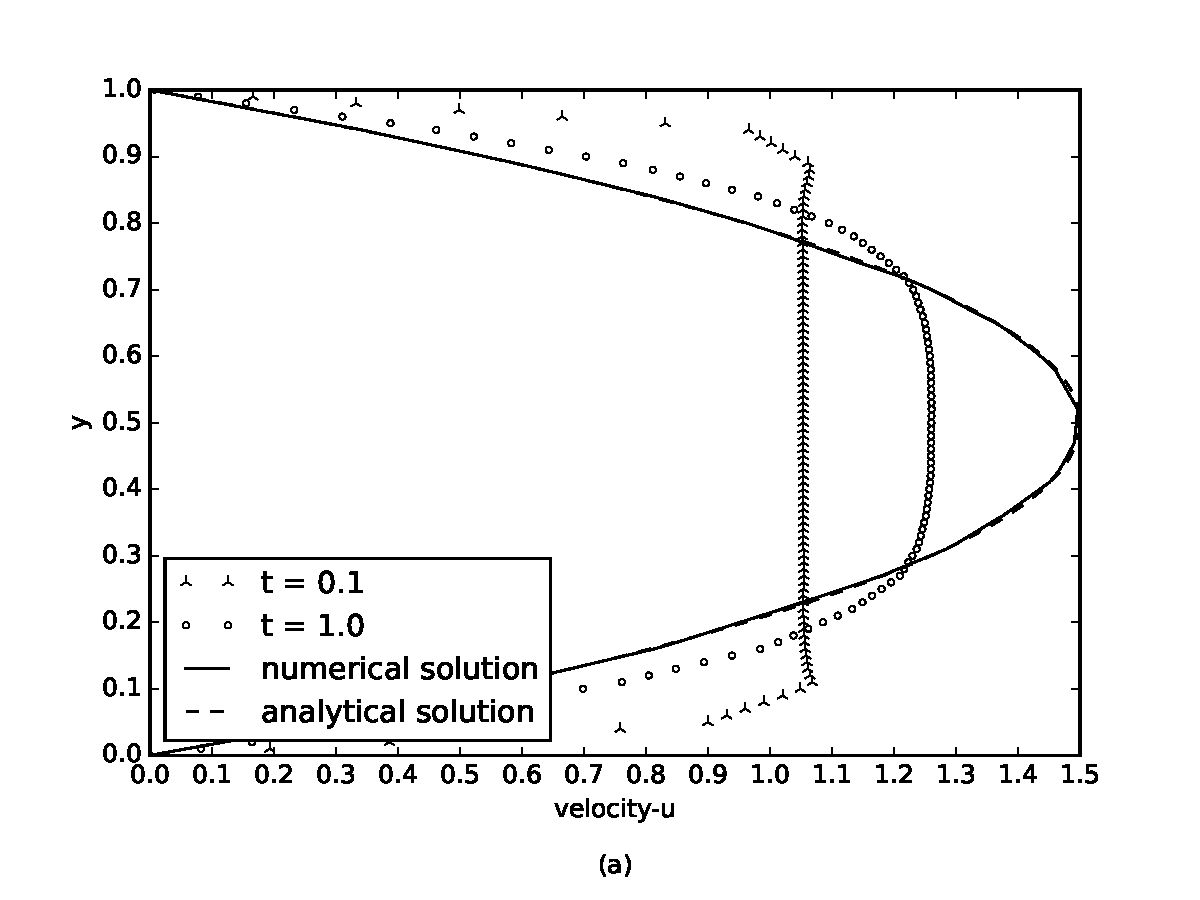
\includegraphics[scale=0.48]{images/poiseuille_velocity.pdf}
\end{figure}
%\vspace{-0.2cm}
%\centering \scriptsize Evolution of velocity field profile in time for \textit{$Re = 100$} and the comparison between numerical solution and analytical solution
\end{column}
\end{columns}
\end{center}
\end{frame}
\fi


%%%%%%%%%%%%%%%%%%%%%%%%%%%%%%%%%%%%%%%%%%%%%%%%%%%%%%%%%%%%%%%%%%%%%%%%%%%%%%%%%%%%%%%%%%

\begin{frame}
 \frametitle{\Large Validation - Poiseuille Flow}
\vspace{-0.55cm}
\begin{center}
\begin{columns}[c]
\begin{column}{0.55\textwidth} 
\small
Boundaries Conditions:\\[0.2cm]
Inflow condition: $u=1$, $v=0$ e $\psi=y$\\[0.1cm]
Outflow condition: $\psi=y$\\[0.1cm]
Top plate: $u=0$, $v=0$, $\psi=1$\\[0.1cm]
Bottom plate: $u=0$, $v=0$, $\psi=0$
\end{column}
\begin{column}{0.35\textwidth} 
\begin{tikzpicture}[scale=0.8]
 \draw [pattern=north east lines] (0,0) -- (0,-0.1) -- (5,-0.1) -- (5,0) -- cycle;
 \draw [pattern=north east lines] (0,1) -- (0,1.1) -- (5,1.1) -- (5,1) -- cycle;
 \draw [dotted] (0,0.9) -- (5,0.9);
 \draw [dotted] (0,0.7) -- (5,0.7);
 \draw [dotted] (0,0.5) -- (5,0.5);
 \draw [dotted] (0,0.3) -- (5,0.3);
 \draw [dotted] (0,0.1) -- (5,0.1);

% \draw [->,thick] (-2,-0.1)--(-2,1.5) node[left] {$y$};
% \draw [->,thick] (-2.1,0)--(-0.5,0) node[below] {$x$};

 \draw  (4.0,0.0) to [bend right=100] (4.0,1.0);
 \draw  (2.5,0.0) to [bend right=100] (2.5,1.0);
 \draw  (1.0,0.0) to [bend right=100] (1.0,1.0);

 \draw [->,thick] (4.0,0.9) to (4.2,0.9);
 \draw [->,thick] (4.0,0.7) to (4.28,0.7);
 \draw [->,thick] (4.0,0.5) to (4.3,0.5);
 \draw [->,thick] (4.0,0.3) to (4.28,0.3);
 \draw [->,thick] (4.0,0.1) to (4.2,0.1);

 \draw [->,thick] (2.5,0.9) to (2.7,0.9);
 \draw [->,thick] (2.5,0.7) to (2.78,0.7);
 \draw [->,thick] (2.5,0.5) to (2.8,0.5);
 \draw [->,thick] (2.5,0.3) to (2.78,0.3);
 \draw [->,thick] (2.5,0.1) to (2.7,0.1);

 \draw [->,thick] (1.0,0.9) to (1.2,0.9);
 \draw [->,thick] (1.0,0.7) to (1.28,0.7);
 \draw [->,thick] (1.0,0.5) to (1.3,0.5);
 \draw [->,thick] (1.0,0.3) to (1.28,0.3);
 \draw [->,thick] (1.0,0.1) to (1.2,0.1);
\end{tikzpicture}
\end{column}
\end{columns}
\end{center}
\vspace{-1.0cm}
\begin{center}
\begin{columns}[c]
\begin{column}{0.55\textwidth} 
\begin{figure}
  \centering
  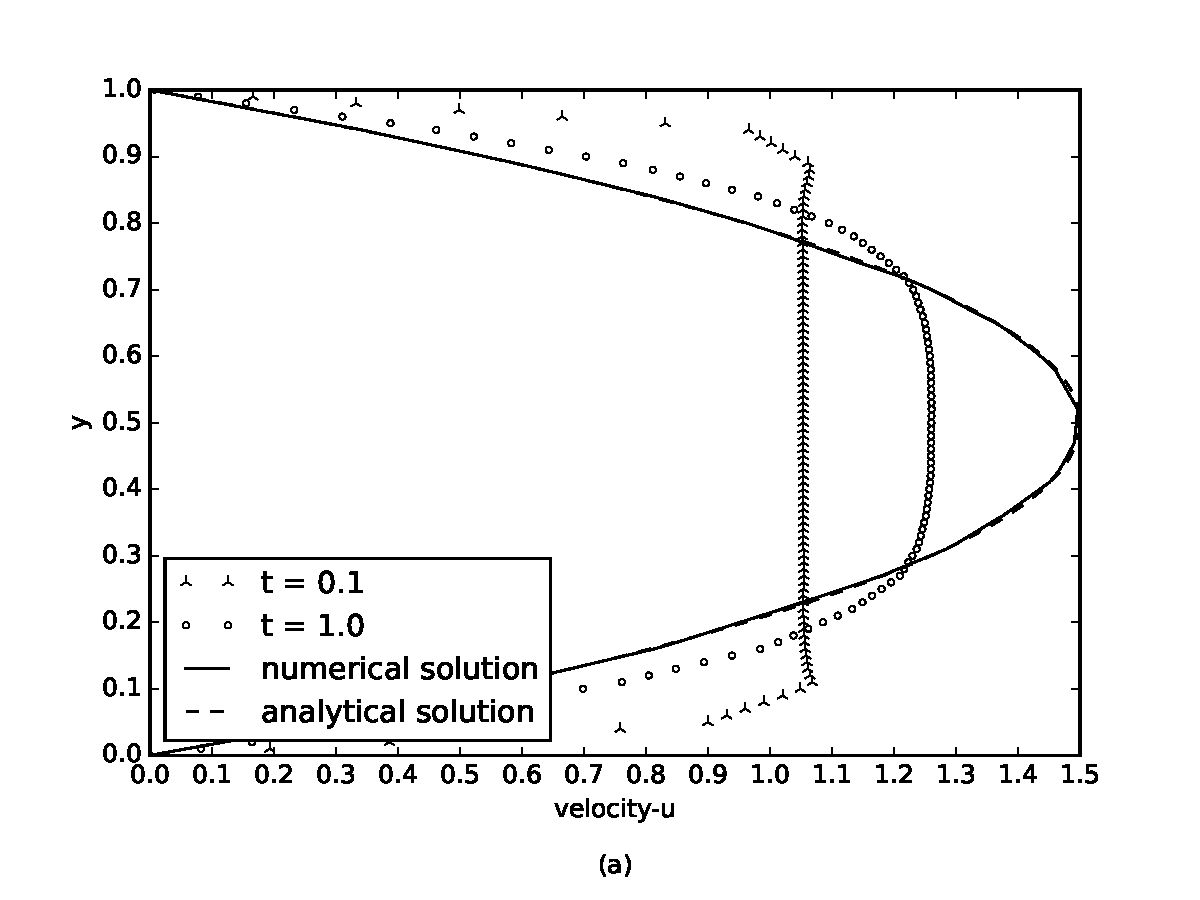
\includegraphics[scale=0.33]{images/poiseuille_velocity.pdf}
\end{figure}
\end{column}
\begin{column}{0.65\textwidth} 
\begin{figure}
  \centering
  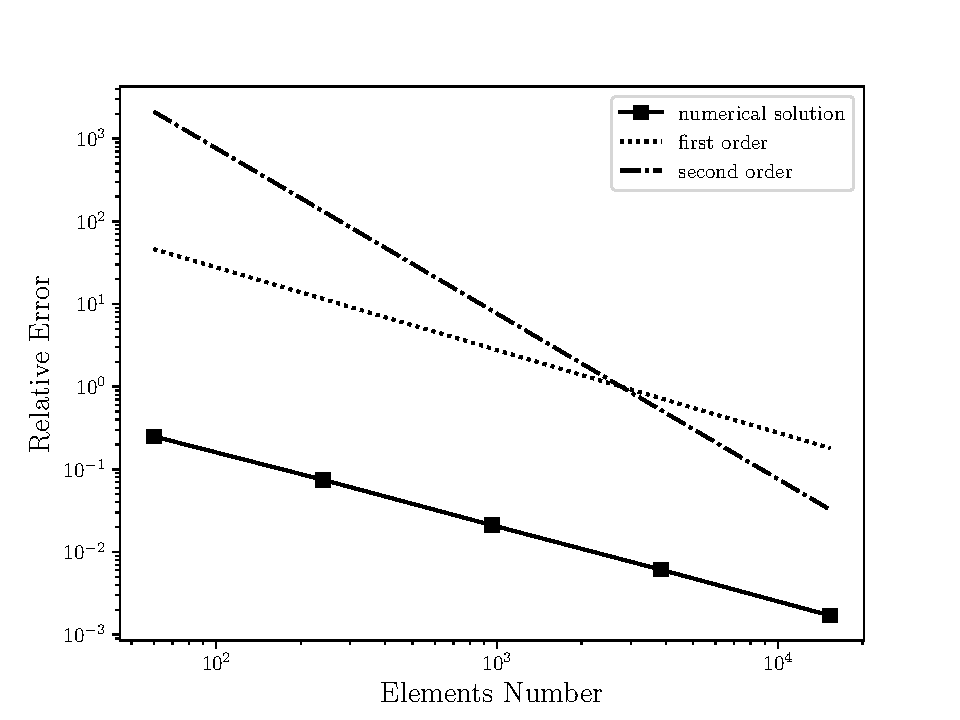
\includegraphics[scale=0.33]{images/poiseuille_error.pdf}
\end{figure}
\end{column}
\end{columns}
\vspace{0.06cm}
\centering \scriptsize (a) comparison of Poiseuille Flow velocity profile and\\ (b) log scale graph of convergence order.
\end{center}
\end{frame}





%%%%%%%%%%%%%%%%%%%%%%%%%%%%%%%%%%%%%%%%%%%%%%%%%%%%%%%%%%%%%%%%%%%%%%%%%%%%%%%%%%%%%%%%%%


\iffalse
\begin{frame}
 \frametitle{\small Validation - Poiseuille Flow}
\begin{figure}
  \centering
  \vspace{-1.5cm}
  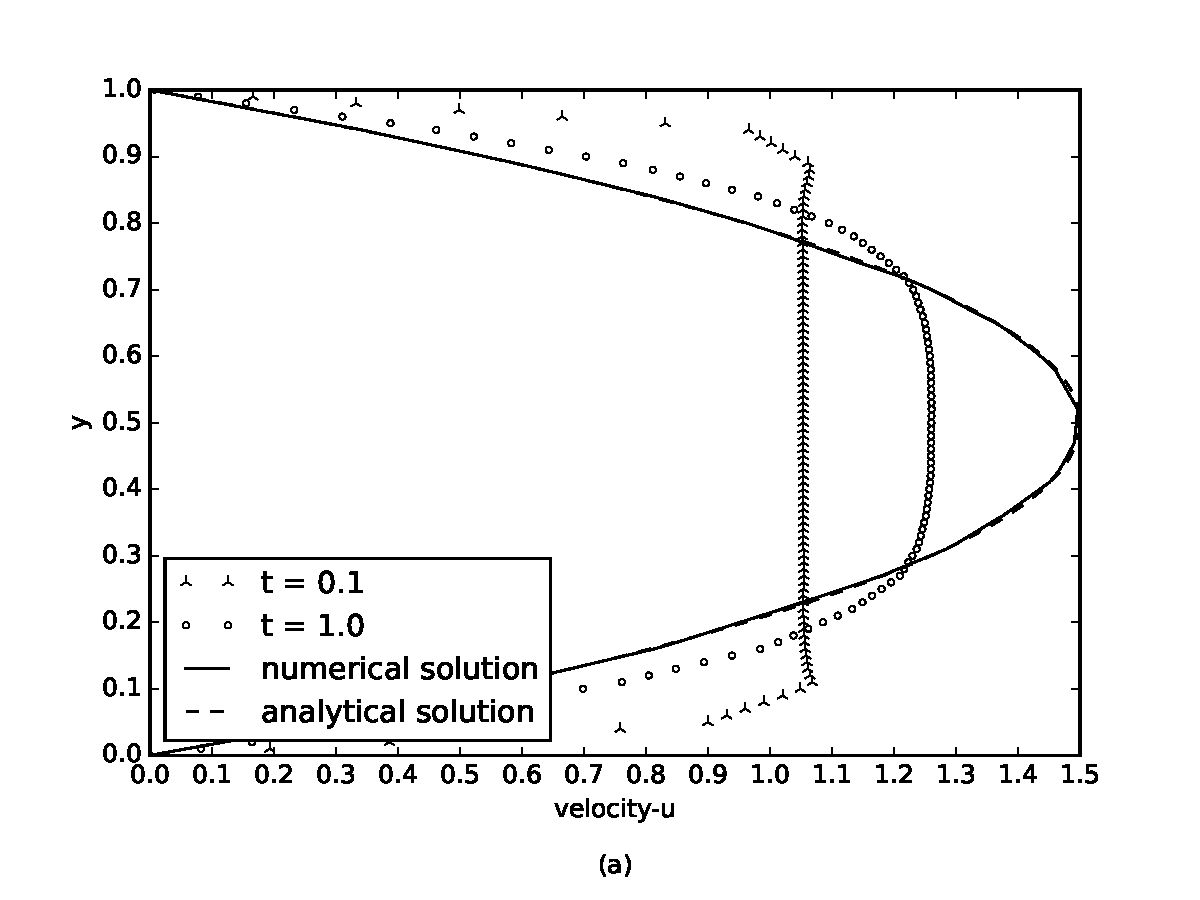
\includegraphics[scale=0.6]{images/poiseuille_velocity.pdf}
\end{figure}
\vspace{-0.2cm}
\centering \scriptsize Evolution of velocity field profile in time for \textit{$Re = 100$} and the comparison between numerical solution and analytical solution.
\end{frame}
\fi

%%%%%%%%%%%%%%%%%%%%%%%%%%%%%%%%%%%%%%%%%%%%%%%%%%%%%%%%%%%%%%%%%%%%%%%%%%%%%%%%%%%%%%%%%%

\begin{frame}
 \frametitle{\Large Validation - Lid Driven Cavity Flow}
\vspace{-1.1cm}
\begin{center}
\begin{columns}[c]
\begin{column}{0.65\textwidth} 
\small
Boundaries Conditions:\\[0.2cm]
Bottom and side plates: $u=0$, $v=0$ e $\psi=0$\\[0.1cm]
Top plate: $u=1$, $v=0$ e $\psi=0$
\end{column}
\begin{column}{0.25\textwidth} 
\begin{tikzpicture}[scale=0.6]
\draw [pattern=north east lines] (0,-0.1) -- (3,-0.1) -- (3,3) -- (2.9,3) -- (2.9,0) -- (0.1,0) -- (0.1,3) -- (0,3) -- cycle;
 \draw [pattern=north east lines] (-0.1,3) -- (-0.1,3.1) -- (3.1,3.1) -- (3.1,3) -- cycle;

 \draw [->,thick] (3.2,3.05)--(4.2,3.05) node[above] {$U_{top}$};

 \draw [->,thick] (2.4,2.4) arc (45:-180:1.2);

% \draw [->,thick] (-2,-0.1)--(-2,1.5) node[left] {$y$};
% \draw [->,thick] (-2.1,0)--(-0.5,0) node[below] {$x$};
\end{tikzpicture}
\end{column}
\end{columns}
\end{center}
\vspace{-0.6cm}
\begin{center}
\begin{columns}[c]
\begin{column}{0.55\textwidth} 
\begin{figure}
  \centering
  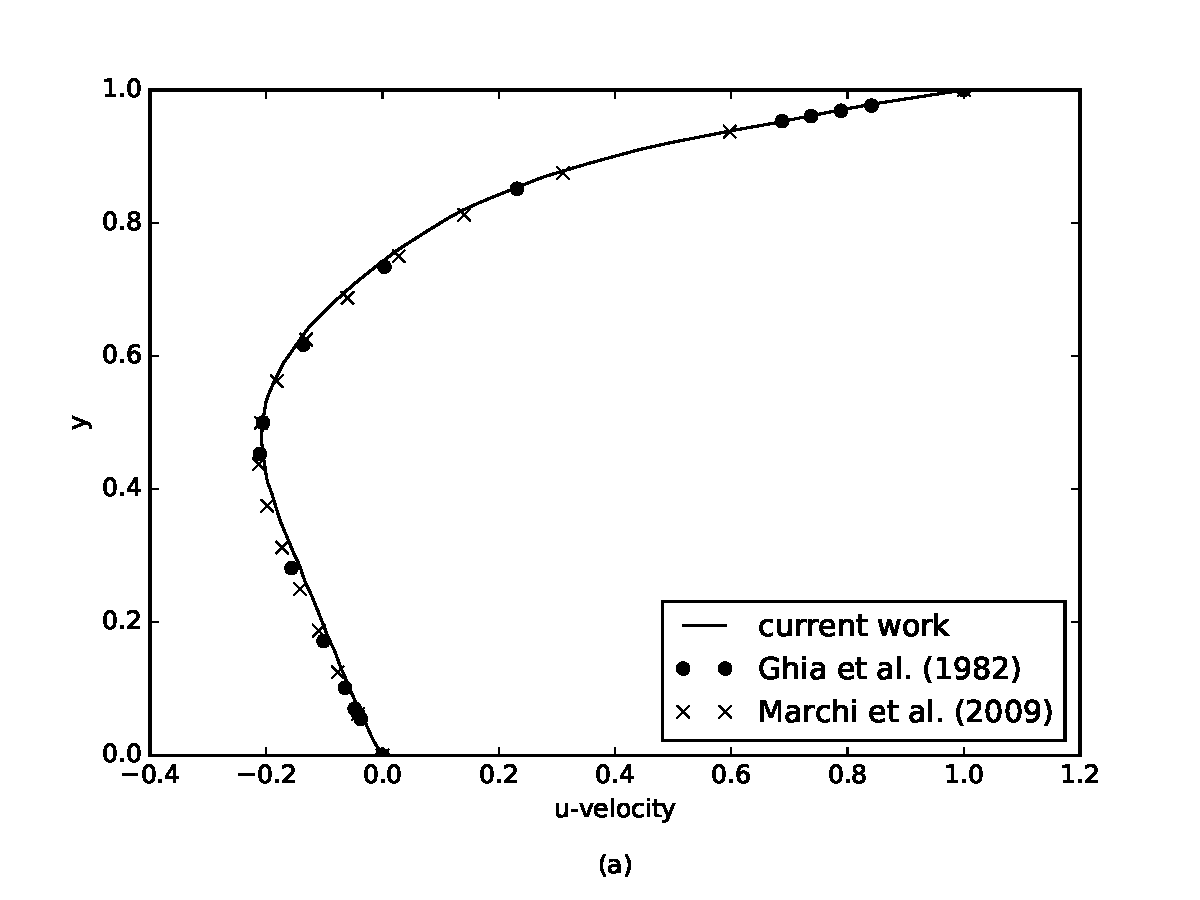
\includegraphics[scale=0.33]{images/Re_100_u_profile.pdf}
\end{figure}
\end{column}
\begin{column}{0.65\textwidth} 
\begin{figure}
  \centering
  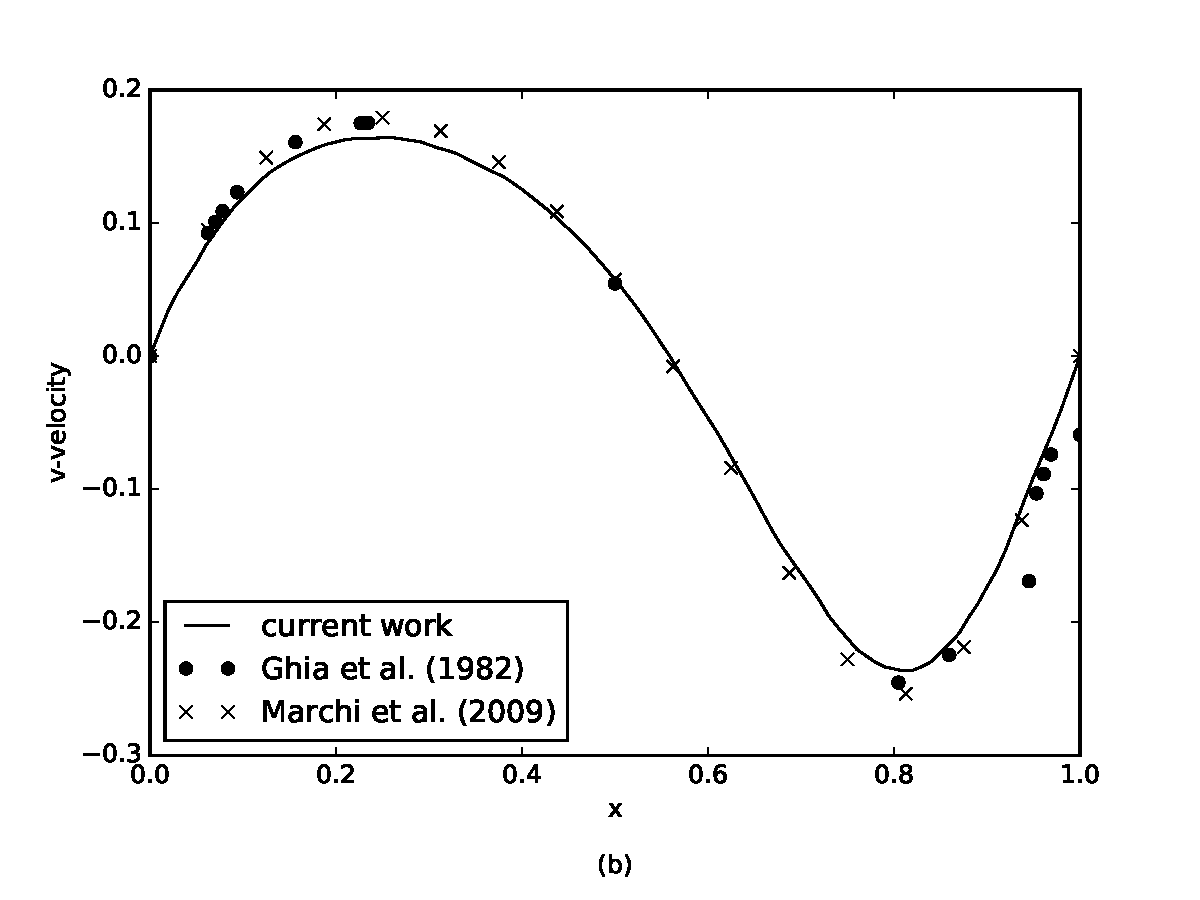
\includegraphics[scale=0.33]{images/Re_100_v_profile.pdf}
\end{figure}
\end{column}
\end{columns}
\vspace{0.1cm}
\centering \scriptsize Centerline velocity profile in a lid-driven cavity for $Re=100$: \\ (a) u-velocity and (b) v-velocity.
\end{center}
\end{frame}



%%%%%%%%%%%%%%%%%%%%%%%%%%%%%%%%%%%%%%%%%%%%%%%%%%%%%%%%%%%%%%%%%%%%%%%%%%%%%%%%%%%%%%%%%%

\iffalse
\begin{frame}
 \frametitle{\small Validation - Lid Driven Cavity Flow}
\vspace{-1cm}
\begin{center}
\begin{tikzpicture}[scale=0.8]
\draw [pattern=north east lines] (0,-0.1) -- (3,-0.1) -- (3,3) -- (2.9,3) -- (2.9,0) -- (0.1,0) -- (0.1,3) -- (0,3) -- cycle;
 \draw [pattern=north east lines] (-0.1,3) -- (-0.1,3.1) -- (3.1,3.1) -- (3.1,3) -- cycle;

 \draw [->,thick] (3.2,3.05)--(4.2,3.05) node[above] {$U_{top}$};

 \draw [->,thick] (2.4,2.4) arc (45:-180:1.2);

% \draw [->,thick] (-2,-0.1)--(-2,1.5) node[left] {$y$};
% \draw [->,thick] (-2.1,0)--(-0.5,0) node[below] {$x$};
\end{tikzpicture}
\end{center}
\vspace{0.5cm}
\small
Boundaries Conditions:\\[0.2cm]
Bottom and side plates: $u=0$, $v=0$ e $\psi=0$;\\[0.1cm]
Top plate: $u=1$, $v=0$ e $\psi=0$
\end{frame}
\fi

%%%%%%%%%%%%%%%%%%%%%%%%%%%%%%%%%%%%%%%%%%%%%%%%%%%%%%%%%%%%%%%%%%%%%%%%%%%%%%%%%%%%%%%%%%

\iffalse
\begin{frame}
 \frametitle{\small Validation - Lid Driven Cavity Flow}
\begin{figure}
  \centering
  \vspace{-1.5cm}
  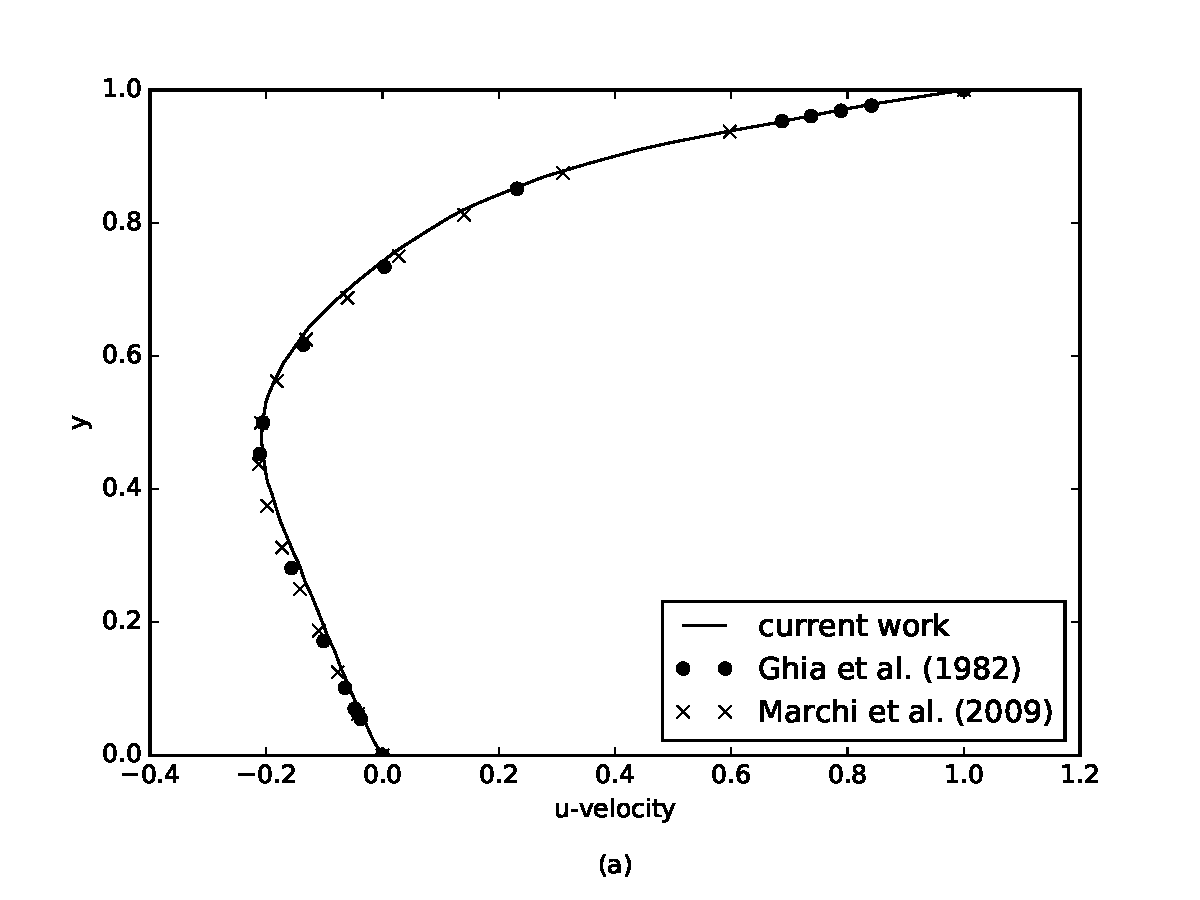
\includegraphics[scale=0.6]{images/Re_100_u_profile.pdf}
\end{figure}
\vspace{-0.2cm}
\centering \scriptsize Centerline $u$ velocity profile ($x=0.5$) in a lid-driven cavity for $Re=100$.
\end{frame}
\fi

%%%%%%%%%%%%%%%%%%%%%%%%%%%%%%%%%%%%%%%%%%%%%%%%%%%%%%%%%%%%%%%%%%%%%%%%%%%%%%%%%%%%%%%%%%
\iffalse
\begin{frame}
 \frametitle{\small Validation - Lid Driven Cavity Flow}
\begin{figure}
  \centering
  \vspace{-1.5cm}
  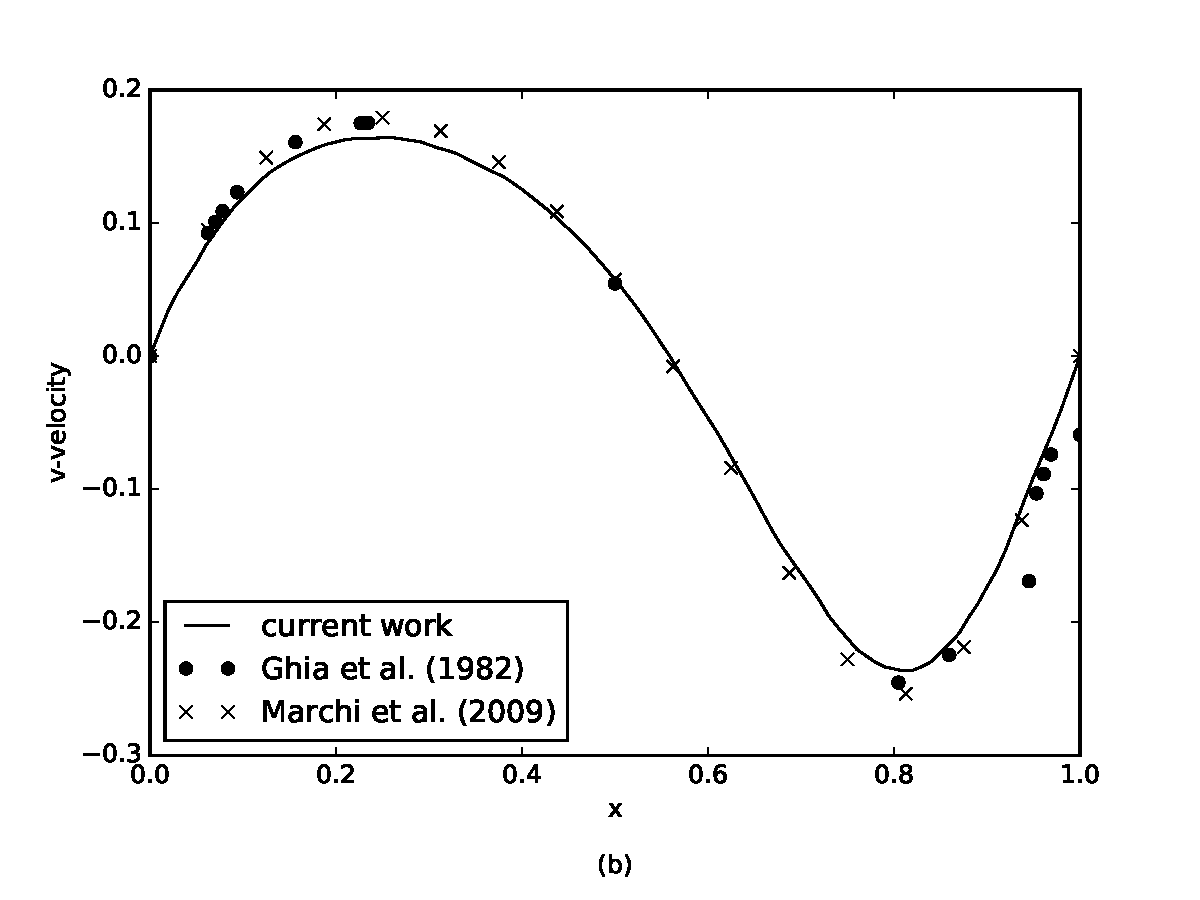
\includegraphics[scale=0.6]{images/Re_100_v_profile.pdf}
\end{figure}
\vspace{-0.2cm}
\centering \scriptsize Centerline $v$ velocity profile ($y=0.5$) in a lid-driven cavity for $Re=100$.
\end{frame}
\fi

%%%%%%%%%%%%%%%%%%%%%%%%%%%%%%%%%%%%%%%%%%%%%%%%%%%%%%%%%%%%%%%%%%%%%%%%%%%%%%%%%%%%%%%%%%

\begin{frame}
  \vspace{-1cm}
  \textcolor{gray}{1. Introduction}\\[0.1cm]
  \textcolor{gray}{2. Mathematical Model}\\[0.1cm]
  \textcolor{gray}{3. Validation}\\[0.1cm]
  4. Results\\[0.1cm]
  \textcolor{gray}{5. Conclusion}
\end{frame}


%%%%%%%%%%%%%%%%%%%%%%%%%%%%%%%%%%%%%%%%%%%%%%%%%%%%%%%%%%%%%%%%%%%%%%%%%%%%%%%%%%%%%%%%%%

\begin{frame}
 \frametitle{\Large Results}
\begin{figure}
  \vspace{-1cm}
     \centering
     \begin{minipage}{.45\linewidth}
      \centering
      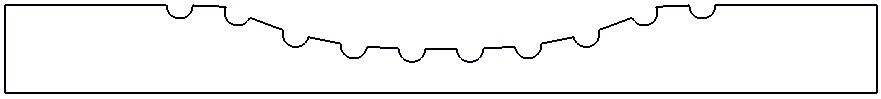
\includegraphics[scale=0.15]{images/CurvedStrut.png}\\
      \scriptsize (a)
     \end{minipage}%
     \begin{minipage}{.45\linewidth}
      \centering
      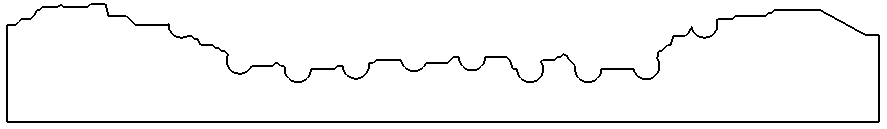
\includegraphics[scale=0.15]{images/RealStrut.png}\\
      \scriptsize (b)
     \end{minipage}
\end{figure}
\vspace{-0.3cm}
\begin{center}
\scriptsize 
     Non-dimensional symmetric geometry for blood flow in coronary artery with drug-eluting stent placed by Wang et al. (2017):
     (a) Curved Channel with Stent
     (b) Real Channel with Stent.
\end{center}
\vspace{0.05cm}
\small
\begin{center}
\begin{columns}[c]
\begin{column}{0.8\textwidth} 
Boundaries Conditions:\\[0.2cm]
Inflow condition: $u=1$, $v=0$ e $\psi=y$;\\[0.1cm]
Outflow condition: $\psi=y$;\\[0.1cm]
Top plate: $u=0$, $v=0$, $\psi=1$;\\[0.1cm]
Symmetry condition: $v=0$, $\psi=0$; \\[0.1cm]
Drug-eluting stent: $u=0$, $v=0$, $\psi=1$ e $c=1$
\end{column}
\hspace{-1cm}
\begin{column}{0.3\textwidth}
$R=0.0015m$\\[0.1cm]
$\mu=0.0035Pa.s$\\[0.1cm]
$\rho=1060kg/m^3$\\[0.1cm]\\
$u=12cm/s$\\[0.1cm]
$Re=54.5$
\end{column}
\end{columns}
\end{center}
\end{frame}


%%%%%%%%%%%%%%%%%%%%%%%%%%%%%%%%%%%%%%%%%%%%%%%%%%%%%%%%%%%%%%%%%%%%%%%%%%%%%%%%%%%%%%%%%%

\iffalse
\begin{frame}
 \frametitle{\Large Results}
\begin{figure}
     \begin{minipage}{.50\linewidth}
      \centering
      
\includegraphics[scale=0.08]{images/vel_RealStrut200.png}\\
      \scriptsize t = 0.1
     \end{minipage}%
     \begin{minipage}{.50\linewidth}
      \centering
      
\includegraphics[scale=0.08]{images/vel_RealStrut1000.png}\\
      \scriptsize t = 0.5
     \end{minipage}
     \begin{minipage}{.50\linewidth}
     \medskip
      \centering
      
\includegraphics[scale=0.08]{images/vel_RealStrut2000.png}\\
      \scriptsize t = 1.0
     \end{minipage}%
     \begin{minipage}{.50\linewidth}
     \medskip
      \centering
      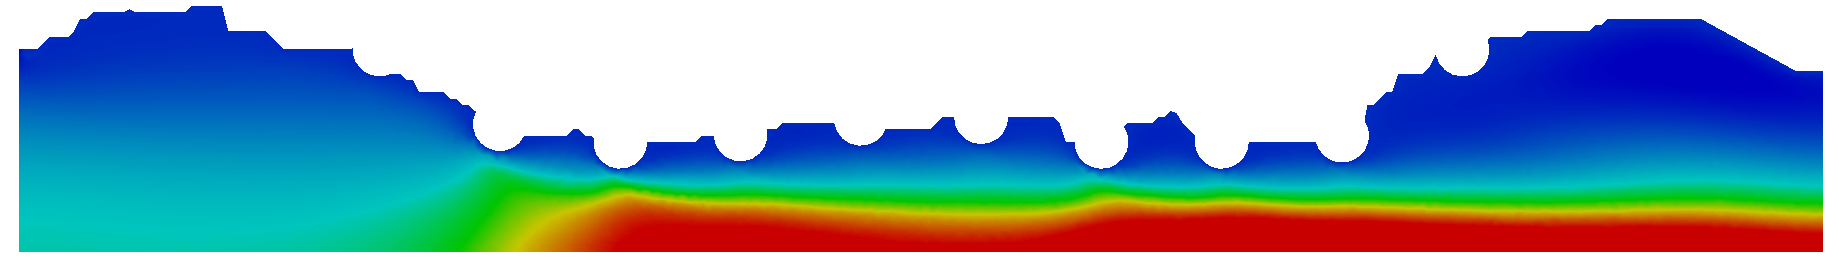
\includegraphics[scale=0.08]{images/vel_RealStrut6000.png}\\
      \scriptsize t = 3.0
     \end{minipage}
     \begin{minipage}{.50\linewidth}
      \centering
      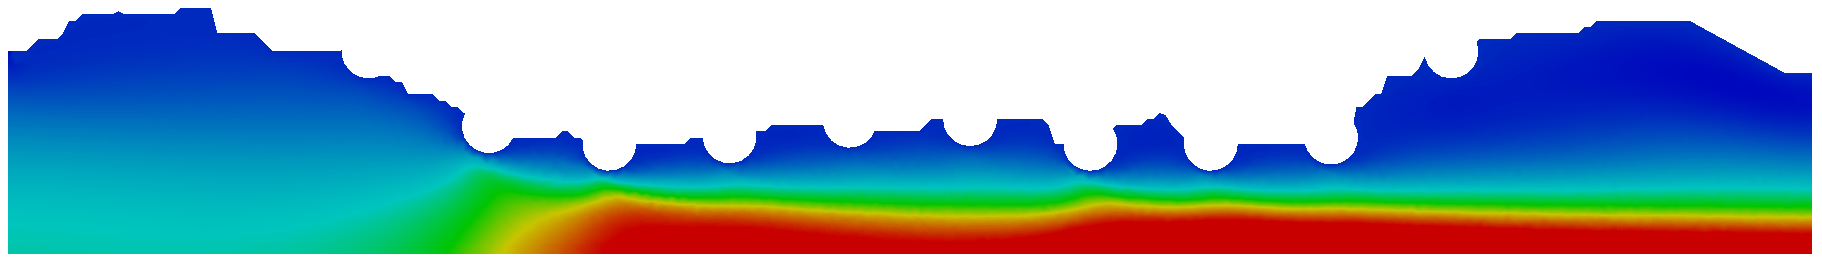
\includegraphics[scale=0.08]{images/vel_RealStrut8000.png}\\
      \scriptsize t = 4.0
     \end{minipage}%
     \begin{minipage}{.50\linewidth}
      \centering
      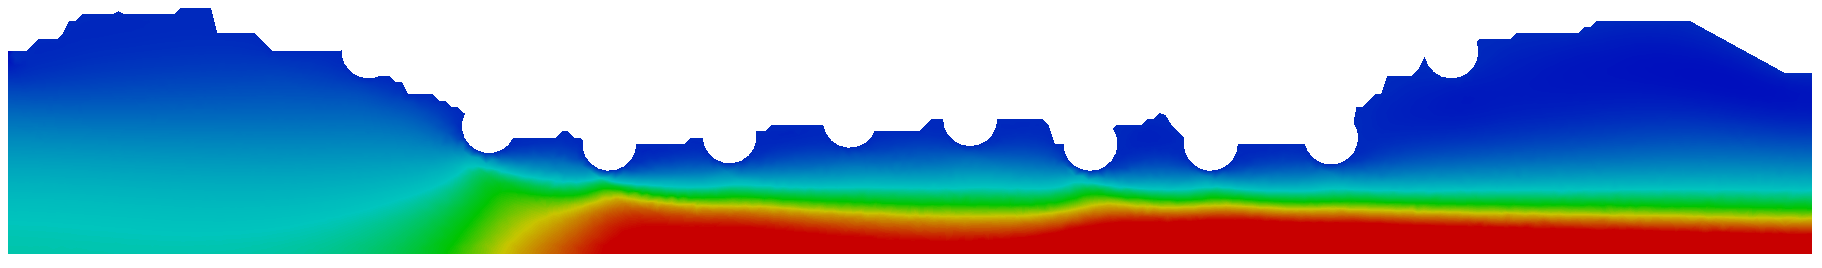
\includegraphics[scale=0.08]{images/vel_RealStrut10000.png}\\
      \scriptsize t = 5.0
 \end{minipage}
     \begin{minipage}{.50\linewidth}
     \medskip
      \centering
      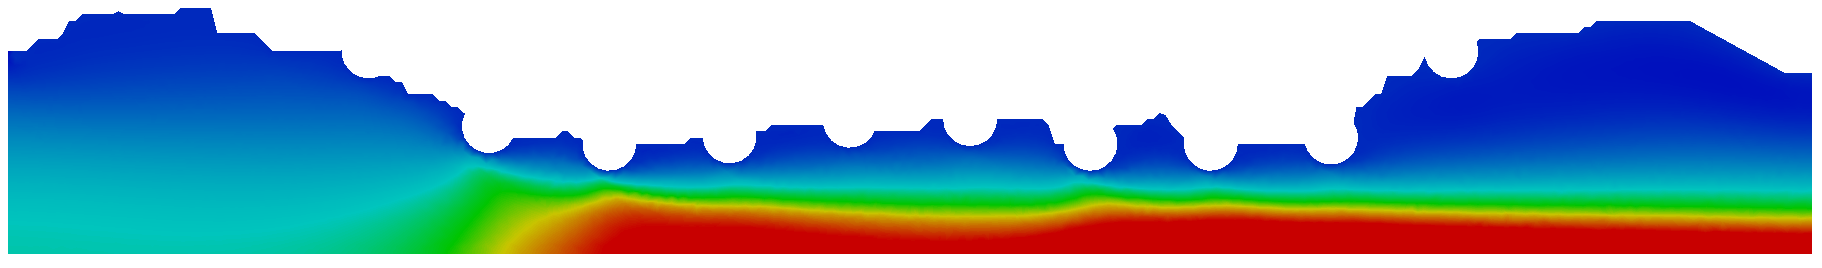
\includegraphics[scale=0.08]{images/vel_RealStrut14000.png}\\
      \scriptsize t = 7.0
     \end{minipage}%
     \begin{minipage}{.50\linewidth}
     \medskip
      \centering
      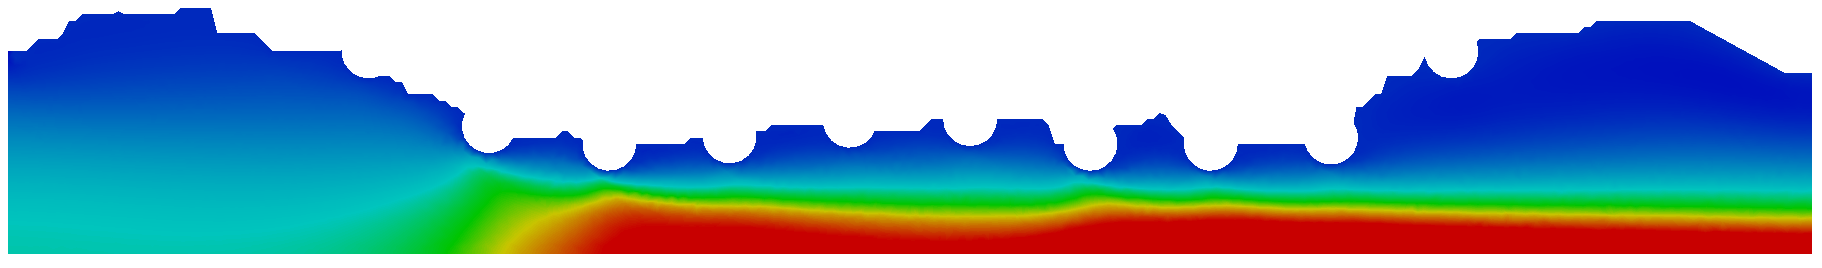
\includegraphics[scale=0.08]{images/vel_RealStrut20000.png}\\
      \scriptsize t = 10.0
     \end{minipage}
\end{figure}
\vspace{0cm}
\centering \scriptsize Evolution in time and space of velocity field
\end{frame}
\fi

%%%%%%%%%%%%%%%%%%%%%%%%%%%%%%%%%%%%%%%%%%%%%%%%%%%%%%%%%%%%%%%%%%%%%%%%%%%%%%%%%%%%%%%%%%

\begin{frame}
 \frametitle{\Large Results - Velocity Field}

\vspace{-0.8cm}
\begin{figure}
     \begin{minipage}{.50\linewidth}
      \centering
      
\includegraphics[scale=0.075]{images/vel_CurvedStrut2000.png}\\
      \tiny t = 1.0
     \end{minipage}%
     \begin{minipage}{.50\linewidth}
      \centering
      
\includegraphics[scale=0.075]{images/vel_RealStrut2000.png}\\
      \tiny t = 1.0
     \end{minipage}
     \begin{minipage}{.50\linewidth}
     \smallskip
      \centering
      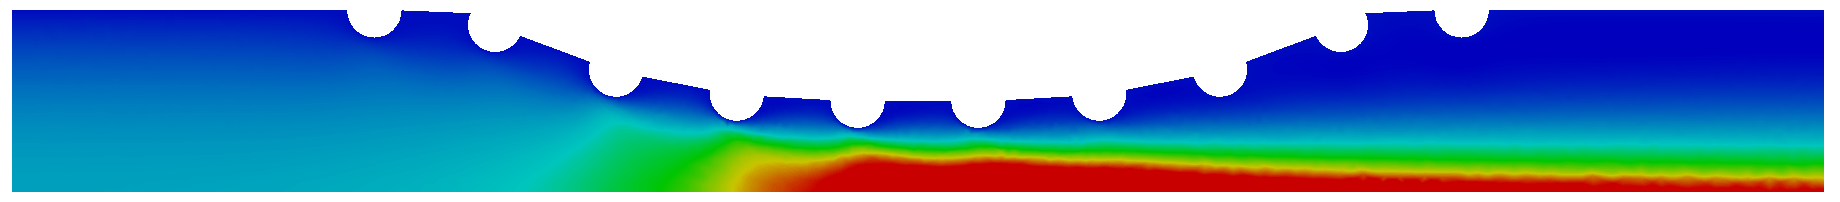
\includegraphics[scale=0.075]{images/vel_CurvedStrut10000.png}\\
      \tiny t = 5.0
     \end{minipage}%
     \begin{minipage}{.50\linewidth}
     \smallskip
      \centering
      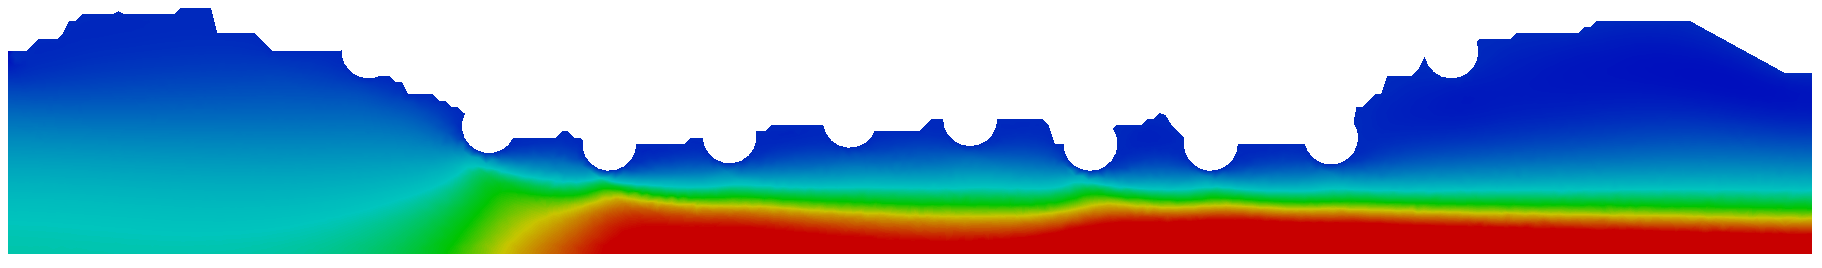
\includegraphics[scale=0.075]{images/vel_RealStrut10000.png}\\
      \tiny t = 5.0
     \end{minipage}
     \begin{minipage}{.50\linewidth}
      \centering
      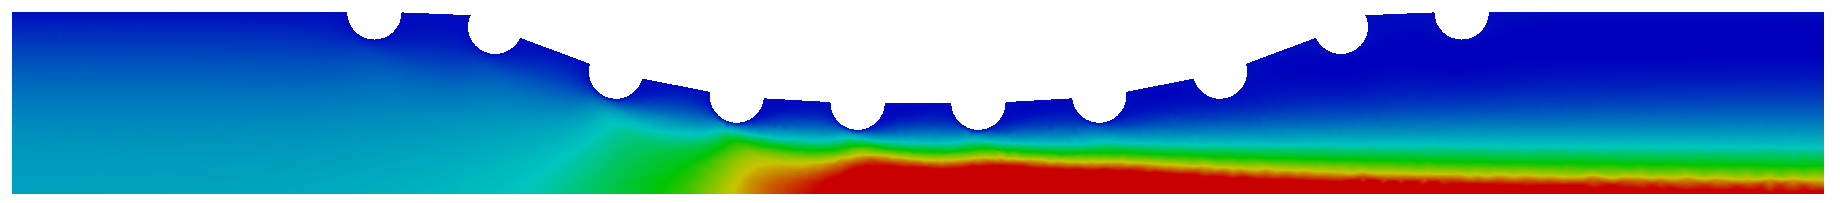
\includegraphics[scale=0.075]{images/vel_CurvedStrut20000.png}\\
      \tiny t = 10.0
     \end{minipage}%
     \begin{minipage}{.50\linewidth}
      \centering
      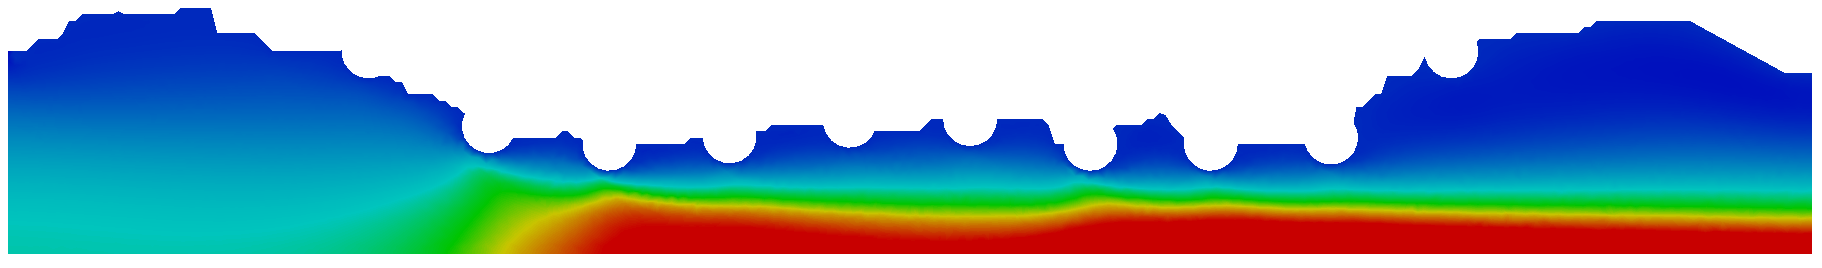
\includegraphics[scale=0.075]{images/vel_RealStrut20000.png}\\
      \tiny t = 10.0
     \end{minipage}
\end{figure}
\vspace{-0.2cm}
\centering \tiny Evolution in time and space of velocity field:\\
                 Curved Channel (left column) and Real Channel (right column)
\vspace{-0.5cm}
\begin{figure}
     \begin{minipage}{.50\linewidth}
     \medskip
      \centering
      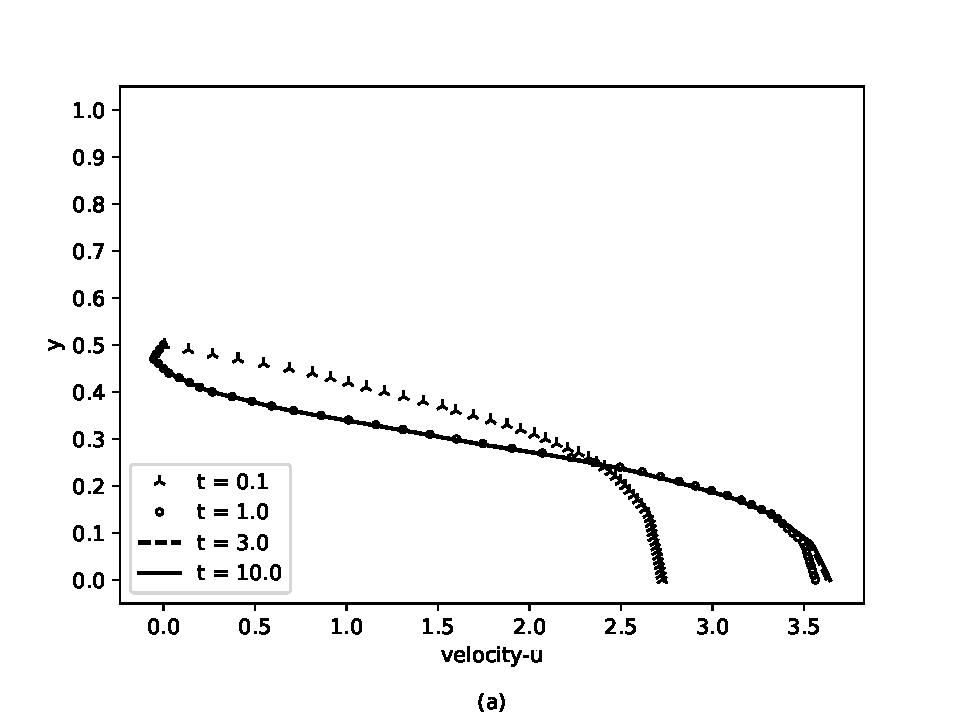
\includegraphics[scale=0.35]{images/vel_CurvedStrut_evol.pdf}\\
     \end{minipage}%
     \begin{minipage}{.50\linewidth}
     \medskip
      \centering
      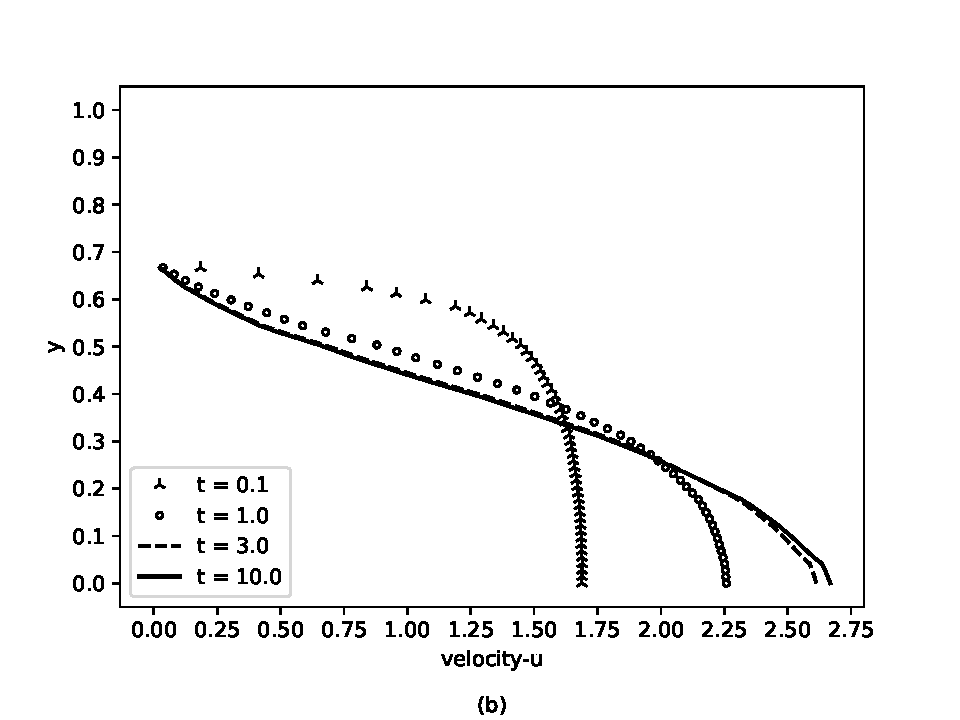
\includegraphics[scale=0.35]{images/vel_RealStrut_evol.pdf}\\
     \end{minipage}
\end{figure}
\vspace{-0.2cm}
\centering \tiny Evolution of velocity profile in centerline ($x=0.5L$):\\
                       (a) Curved Channel and (b) Real Channel
\end{frame}

%%%%%%%%%%%%%%%%%%%%%%%%%%%%%%%%%%%%%%%%%%%%%%%%%%%%%%%%%%%%%%%%%%%%%%%%%%%%%%%%%%%%%%%%%%

\begin{frame}
 \frametitle{\Large Results - Concentration Field}
\vspace{-0.7cm}
\begin{figure}
     \begin{minipage}{.50\linewidth}
      \centering
      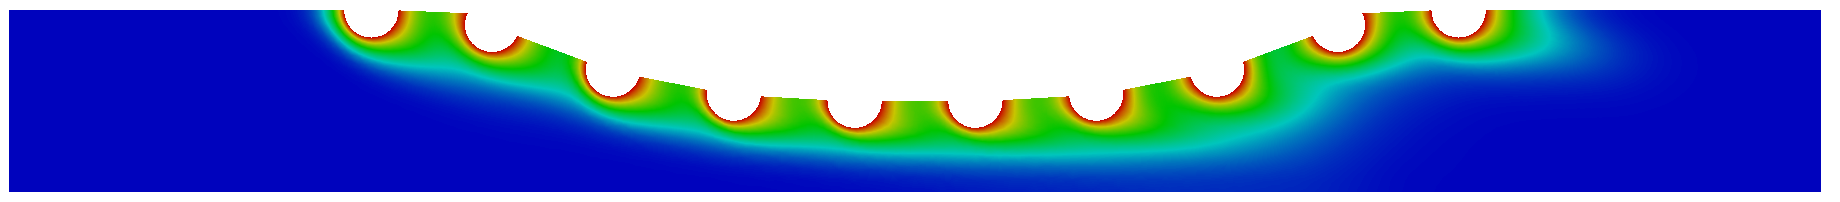
\includegraphics[scale=0.075]{images/conc1_CurvedStrut2000.png}\\
      \tiny t = 1.0
     \end{minipage}%
     \begin{minipage}{.50\linewidth}
      \centering
      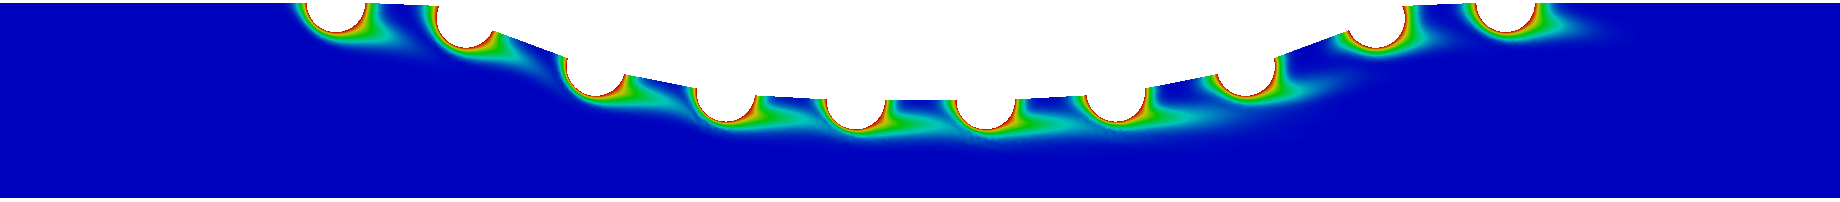
\includegraphics[scale=0.075]{images/conc10_CurvedStrut5000.png}\\
      \tiny t = 1.0
     \end{minipage}
     \begin{minipage}{.50\linewidth}
     \medskip
      \centering
      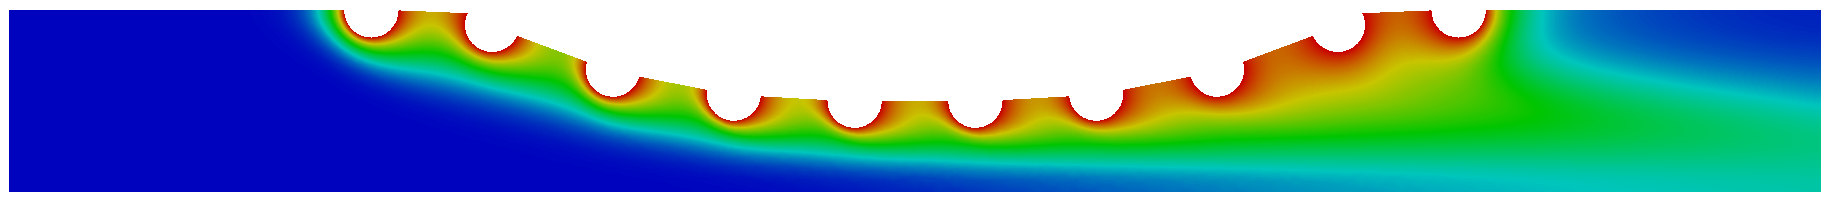
\includegraphics[scale=0.075]{images/conc1_CurvedStrut10000.png}\\
      \tiny t = 5.0
     \end{minipage}%
     \begin{minipage}{.50\linewidth}
     \medskip
      \centering
      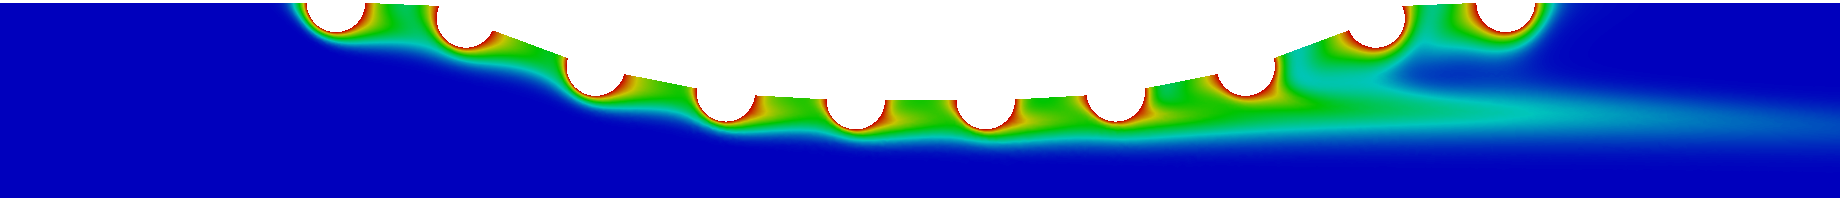
\includegraphics[scale=0.075]{images/conc10_CurvedStrut25000.png}\\
      \tiny t = 5.0
     \end{minipage}
     \begin{minipage}{.50\linewidth}
      \centering
      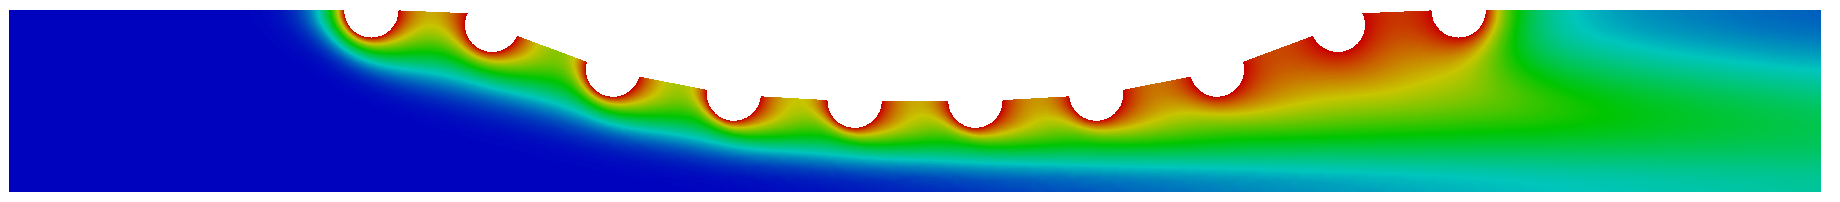
\includegraphics[scale=0.075]{images/conc1_CurvedStrut20000.png}\\
      \tiny t = 10.0
     \end{minipage}%
     \begin{minipage}{.50\linewidth}
      \centering
      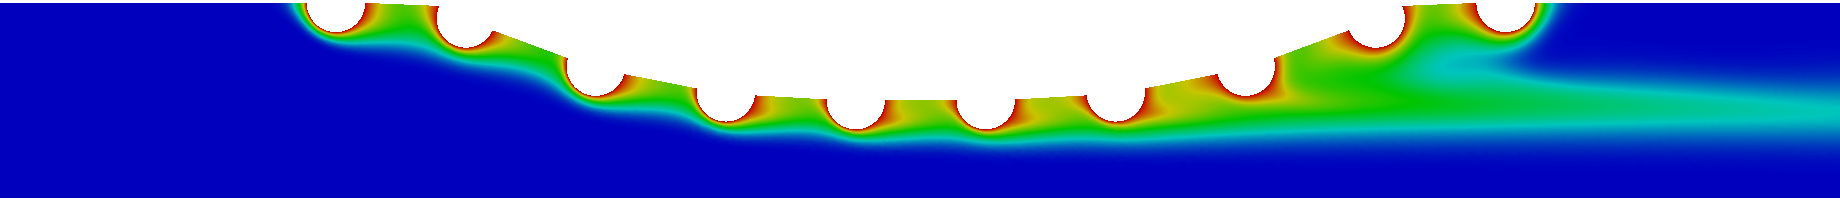
\includegraphics[scale=0.075]{images/conc10_CurvedStrut50000.png}\\
      \tiny t = 10.0
     \end{minipage}
\end{figure}
\vspace{-0.2cm}
\centering \scriptsize Evolution in time and space of concentration field in Curved Channel:\\
                 $Sc=1$ (left column) and $Sc=10$ (right column)
\vspace{0cm}
\begin{figure}
     \begin{minipage}{.50\linewidth}
      \centering
      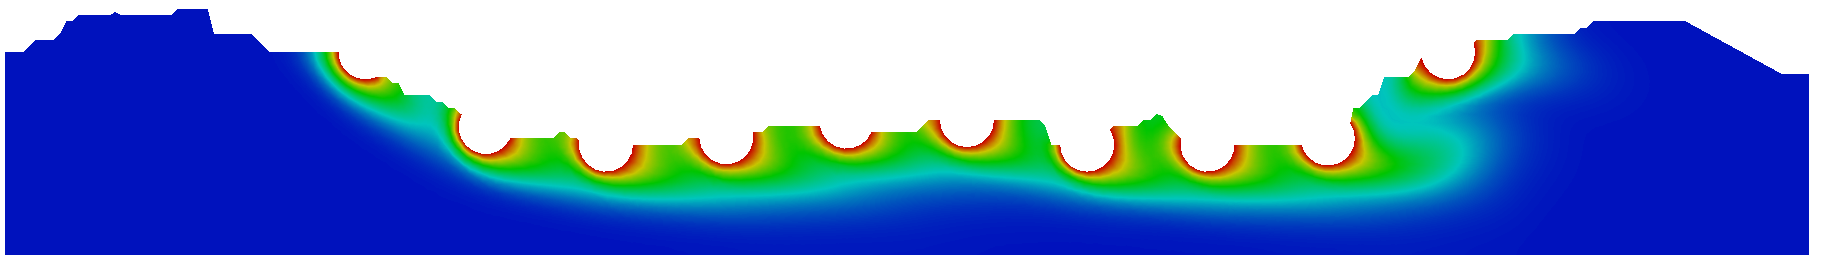
\includegraphics[scale=0.075]{images/conc1_RealStrut2000.png}\\
      \tiny t = 1.0
     \end{minipage}%
     \begin{minipage}{.50\linewidth}
      \centering
      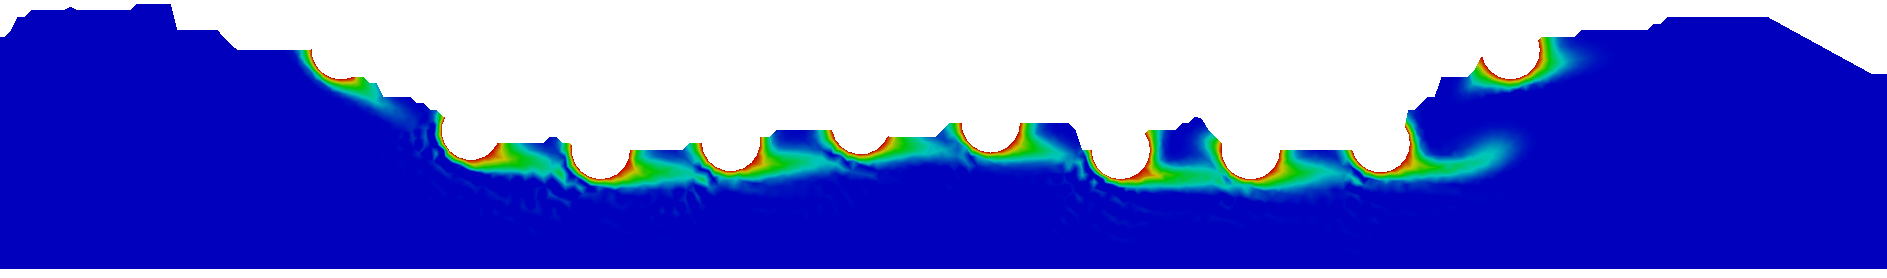
\includegraphics[scale=0.075]{images/conc10_RealStrut5000.png}\\
      \tiny t = 1.0
     \end{minipage}
     \begin{minipage}{.50\linewidth}
     \medskip
      \centering
      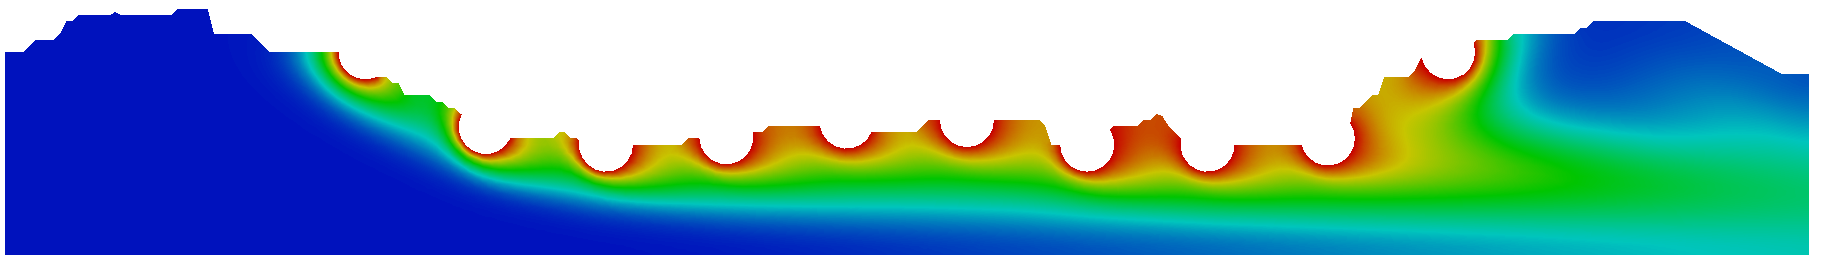
\includegraphics[scale=0.075]{images/conc1_RealStrut10000.png}\\
      \tiny t = 5.0
     \end{minipage}%
     \begin{minipage}{.50\linewidth}
     \medskip
      \centering
      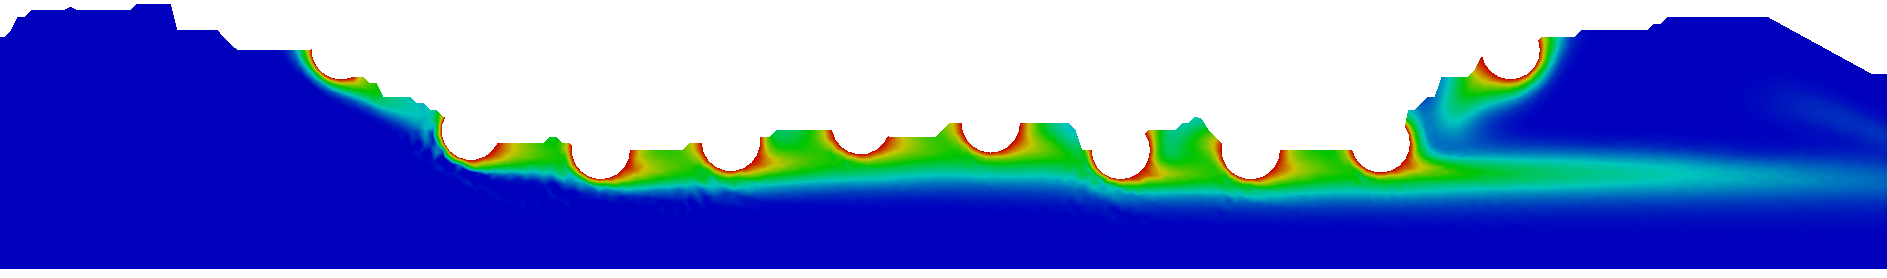
\includegraphics[scale=0.075]{images/conc10_RealStrut25000.png}\\
      \tiny t = 5.0
     \end{minipage}
     \begin{minipage}{.50\linewidth}
      \centering
      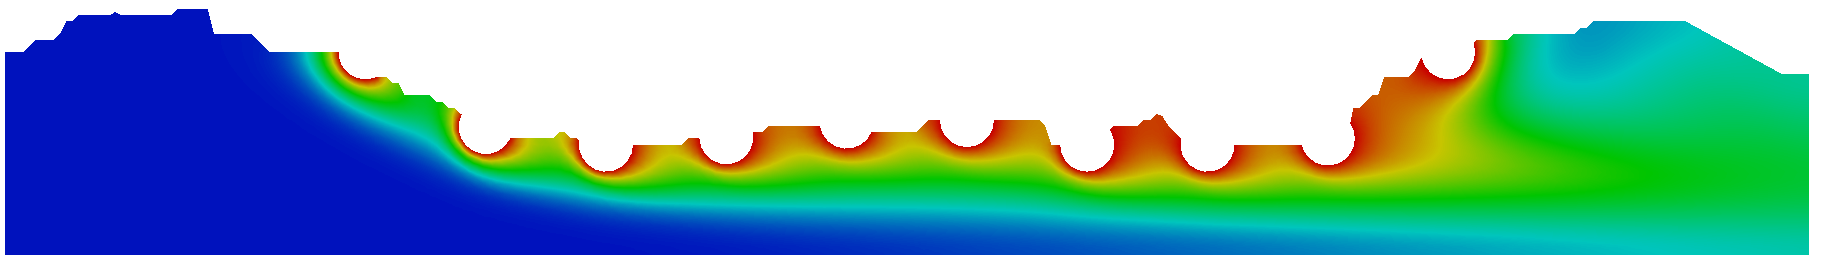
\includegraphics[scale=0.075]{images/conc1_RealStrut20000.png}\\
      \tiny t = 10.0
     \end{minipage}%
     \begin{minipage}{.50\linewidth}
      \centering
      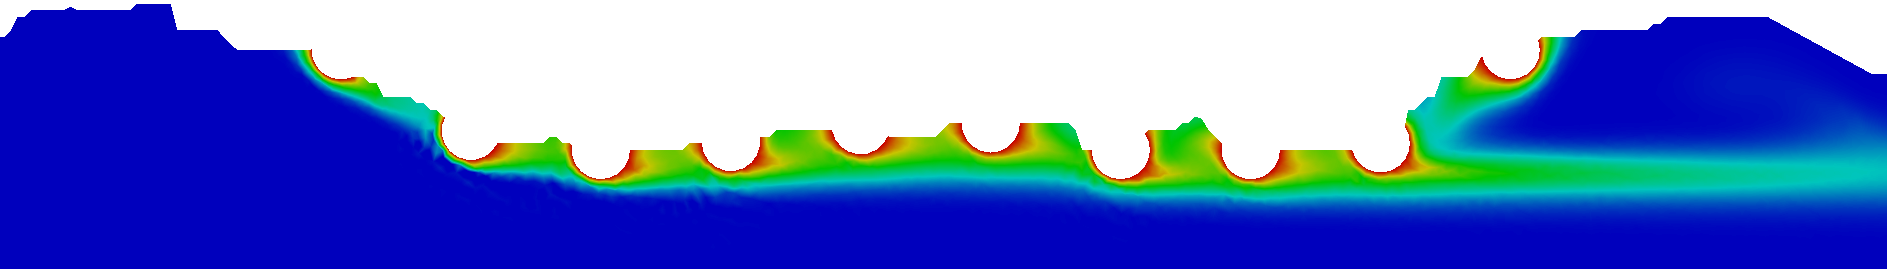
\includegraphics[scale=0.075]{images/conc10_RealStrut50000.png}\\
      \tiny t = 10.0
     \end{minipage}
\end{figure}
\vspace{-0.2cm}
\centering \scriptsize Evolution in time and space of concentration field in Real Channel:\\
                 $Sc=1$ (left column) and $Sc=10$ (right column)
\end{frame}


%%%%%%%%%%%%%%%%%%%%%%%%%%%%%%%%%%%%%%%%%%%%%%%%%%%%%%%%%%%%%%%%%%%%%%%%%%%%%%%%%%%%%%%%%%

\begin{frame}
  \vspace{-1cm}
  \textcolor{gray}{1. Introduction}\\[0.1cm]
  \textcolor{gray}{2. Mathematical Model}\\[0.1cm]
  \textcolor{gray}{3. Validation}\\[0.1cm]
  \textcolor{gray}{4. Results}\\[0.1cm]
  5. Conclusion
\end{frame}


%%%%%%%%%%%%%%%%%%%%%%%%%%%%%%%%%%%%%%%%%%%%%%%%%%%%%%%%%%%%%%%%%%%%%%%%%%%%%%%%%%%%%%%%%%

\begin{frame}
 \frametitle{\Large Conclusion}
 \vspace{-1cm}
\begin{enumerate}
 \justifying
 \small
 \item Was observed that the species transport in blood flow is directly influenced
       by drug used in stent production\\

 \vspace{0.3cm}
 
 \item The streamfunction-vorticity formulation showed an useful approach for to calculate
       the velocity and concentration fields since the variables are scalars allowing a
       smooth implementation\\

 \vspace{0.3cm}

 \item Due to generalized construction of the code, the simulator is able to describe
       drug-eluting stent problem in coronary artery as well as flows of Newtonian fluids
       with scalar transport (concentration or temperature)
\end{enumerate}
\end{frame}


%%%%%%%%%%%%%%%%%%%%%%%%%%%%%%%%%%%%%%%%%%%%%%%%%%%%%%%%%%%%%%%%%%%%%%%%%%%%%%%%%%%%%%%%%%

\begin{frame}
 \centering
 \vspace{-1cm}
 \Huge Thank you!\\
 \vspace{0.5cm}
 \small marquesleandro67@gmail.com\\
 \small gustavo.anjos@uerj.br\\
 \small jose.pontes@uerj.br\\
 \vspace{1.0cm}
 \small The authors thank the FAPERJ (Research Support Foundation of the State of Rio de Janeiro)
        for its financial support

 \vspace{-0.2cm}
 \begin{figure}
  \centering
  
\includegraphics[scale=0.4]{images/faperj.jpg}\\
 \end{figure}
\end{frame}




\end{document}
%%%%%%%%%%%%%%%%%%%%%%%%%%%%%%%%%%%%%%%%%%%%%%%%%%%%%%%%%%%%%%%%%%%%%%%%%%%%%%%%%%%%%%%%%%
